\chapter{Schleifen}
\epigraph{
	Insanity: doing the same thing over and over again and expecting different results
}{Albert Einstein}

Computer können dazu benutzt werden, die immer gleichen (lästigen) Aufgaben wiederholt und in schneller Folge auszuführen. Es ist möglich, bei jeder Wiederholung einen einzelnen Eingabewert zu ändern und so \eg Berechnungen für einen ganzen Wertebereich durchzuführen, oder Messwerte von einem Gerät zu überwachen.

Zeichnet man ein \emph{Flussdiagramm} eines solchen Programms (wie in Abbildung \ref{fig:FlowBasicLoop}), so findet sich in der Regel ein Programmteil, der zur Vorbereitung dient und in gewohnter Weise \enquote{von oben nach unten} abgearbeitet wird. An diesen schließt sich ein Abschnitt an, der einige Male wiederholt werden soll, und daher im Flussdiagramm als Bogen dargestellt wird. Nach diesem Teil könnte die Ausgabe der Ergebnisse stattfinden, die wiederum in gewohnter \emph{linearer} Weise (also von oben nach unten) bearbeitet wird. 

Die Form dieses Flussdiagramms motiviert den Namen \emph{Schleife} für eine solche Struktur.

\begin{figure}[h!]
\begin{center}
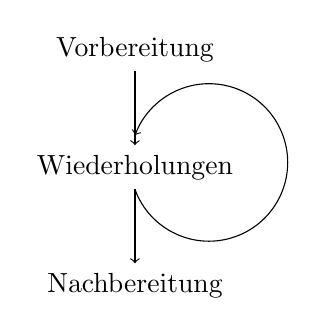
\begin{tikzpicture}
    \node at (0, 3  ) (Input)      {Vorbereitung};
    \node at (0, 1.5) (Operations) {Wiederholungen};
    \node at (0, 0  ) (Output)     {Nachbereitung};
    
    \draw [->] (Input) -- (Operations);
    \draw [->] (Operations.south)arc(-160:160:1.0);		%start angle: stop angle : radius
    \draw [->] (Operations) -- (Output);
\end{tikzpicture}
\caption{Programmflussdiagramm mit Schleife} \label{fig:FlowBasicLoop}
\end{center}
\end{figure}

In der Regel ist die Zahl der Schleifendurchläufe an eine Bedingung geknüpft; genauso sind aber auch \emph{Endlosschleifen} möglich. In diesem Kapitel werden wir verschiedene Schleifentypen und ihre Anwendungsfelder kennen lernen.

\begin{hintbox}[Laufende Programme zum Beenden zwingen: \texttt{STRG + C}]
Macht man einen Fehler bei der Formulierung der Bedingung, so kann man unbeabsichtigt eine Endlosschleife erstellen. Ein solches Programm wird von sich selbst aus nie beendet. Wir können zu jeder Zeit aber das Beenden erzwingen, indem wir in der Konsole die Tastenkombination \texttt{STRG + C} drücken.
\end{hintbox}

\section{\inPy{while}-Loops}
break; else (code on non-entry)

\begin{hintbox}[Garantierte erste Ausführung]
\begin{minted}[linenos]{python}
while True:
  stuff()
  if fail_condition:
    break
\end{minted}
\end{hintbox}

    
\section{\inPy{for}-Loops}
\begin{hintbox}[Falls Sie von einer anderen Sprache kommen: Keine Indices]
x
\end{hintbox}

\begin{hintbox}[Objekt und Index: \texttt{enumerate}]
x
\end{hintbox}

\begin{hintbox}[Underscore]
normally last result; in code usually obligatory forget.
\end{hintbox}

\section{List Comprehension}
can be used in lists, tuples, dicts, sets, ...